\chapter{Einleitung}
Jeder Bericht beginnt mit einer Einleitung. In diesem Abschnitt muss man den Leser sanft auf die behandelte Thematik einstimmen. Dabei wird der allgemeine Kontext des Projektes genau beschrieben ohne speziell auf Details einzugehen.


%---------------------------------------------------------
\section{Aufgabenstellung}
In diesem Abschnitt erfolgt eine Beschreibung der Aufgabenstellung. Es ist darzustellen, wie die Aufgabe lautet oder was untersucht werden soll. Hier ist eine detailliere Beschreibung der Aufgabe gefordert.

%---------------------------------------------------------
\section{Pflichtenheft}
Eine genaue Definition, was in diesem Projekt alles realisiert werden soll ist Gegenstand dieses Abschnitts. Dabei soll unterschieden werden, welche Bestandteile Pflicht und welche optional sind. Dieser Abschnitt ist weniger relevant, wenn es sich um eine Master Thesis handelt, die einen wissenschaftlichen Charakter besitzt. In allgemeinen Projekten ist er Pflicht. Die einzelnen Arbeitspunkte sind bei einem Projekt mit mehreren Personen dem einzelnen Projektmitarbeiter zuzuordnen.

%---------------------------------------------------------
\section{Zeitplan}
Jede Projektplanung beinhaltet zwingend einen Zeitplan. Dabei wird angegeben, welche Zeit f�r die Arbeit zur Verf�gung steht und wie diese Zeit in Abh�ngigkeit von der Aufgabe und dem Pflichtenheft eingeteilt wird. Der Zeitplan kann in Textform (Tabelle) oder in grafischer Form dargestellt werden. In Abh�ngigkeit von dem Umfang der Arbeit und der vorhandenen Zeit ist dieser zu gliedern. Als Werkzeug f�r die Erstellung bietet sich das Programm \index{VISIO} von Microsoft an. Sind mehrere Personen an dem Projekt beteiligt, so ist auch dies im Zeitplan darzustellen. In Abbildung \vref{fig:zeitplan} ist eine Zeitplan dargestellt.
\begin{figure}[htbp]
	\centering
		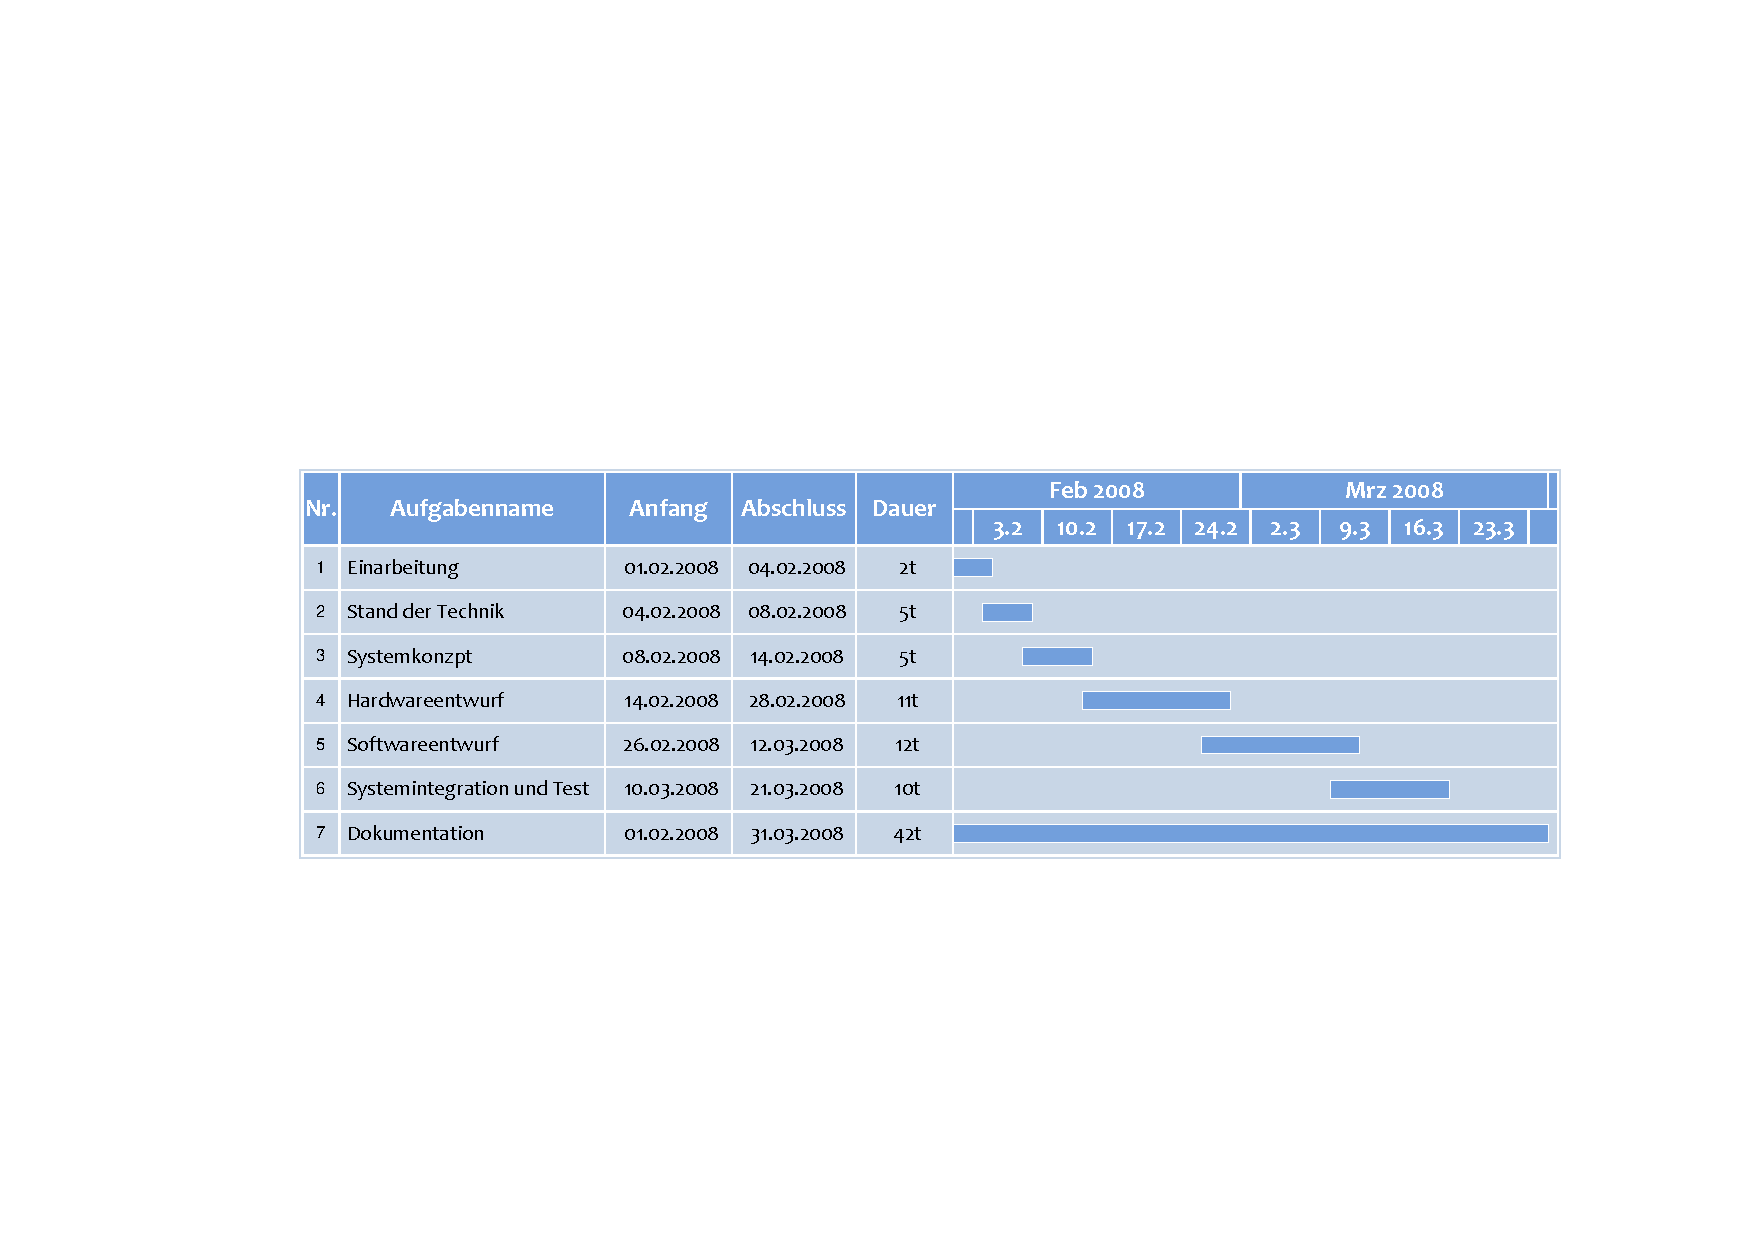
\includegraphics[width=\textwidth]{Bilder/zeitplan_v1.pdf}
	\caption{Beispiel eines Zeitplans}
	\label{fig:zeitplan}
\end{figure}

F�r die Absch�tzung der Dauer der Dokumentation k�nnen Sie davon ausgehen, dass Sie im g�nstigsten Fall pro Tag zwei bis vier Seiten Text, der in die Endfassung eingeht, erstellen k�nnen. Denken Sie jedoch daran: kein Mensch kann jeden Tag schreiben! Neben diversen anderen Unw�gbarkeiten und immer mal wieder auftretenden Konzentrationshindernissen k�nnen z.~B. �berarbeitungen oder weitere Untersuchungen notwendig werden, um die beim Abfassen der Arbeit neu auftauchenden Fragen beantworten zu k�nnen.


%---------------------------------------------------------
\section{Gliederung der Arbeit}
Die Aufgabe dieses Abschnitts ist die Darstellung der Struktur der Ausarbeitung. Es ist die Frage zu beantworten, was enthalten die weiteren Kapitel? 